\documentclass{article}
\usepackage[utf8]{inputenc}
\usepackage{url}
\usepackage{graphicx}
\usepackage{hyperref}

\begin{document}
\title{Facial Recognition Project}
\begin{figure}
    \centering
    
\includegraphics[scale = 0.5]{gmit}
    \label{fig:gmit}
\end{figure}
\author{Arnas Steponavicius
        \and Aaron Moran
        \and Thomas Kenny}
\date{\today}

\maketitle
\section{Introduction}
When we formed our team there was many ideas floating around of what to design and make. We tried to think of an idea that was new and exciting for the three of us. We wanted to make design and make something that was challenging and would improve our ability as software students. The idea we settled on was Facial Recognition. 
    
With extensive research into this field we looked at many languages to use. We thought it would be a good idea to learn a new language while working on this project. This language was Python. 
Python is one of the top languages used worldwide at the moment so we thought this would be beneficial for us to learn this language. We chose this language for various reasons, one of these reasons being that there is various packages python offers. We found online that there is a library called \textbf{face\_recognition} that suited our needs for this project. 

We had various meetings in the beginning to find the pros and cons of Facial Recognition. We had to map out the project and treat this like it was a job. This included making a plan of what we wanted to have done to present in our weekly meetings, breaking up the project into steps so we wouldn't’t get overwhelmed or held up on one task and discussing what each member of the team would focus on. Each task will be explained in further detail.

GitHub was vital with our project. It was important that we constantly used GitHub to display the progress we were making. We could handle issues we were having, test different ideas and we could all be on the same page as we work.

\maketitle
\section{System Requirements}
\textbullet{ Python 3.x } \newline
\textbullet{ C/C++ compiler installed }\newline
\textbullet{ CMake \url{https://cmake.org/download/ }}\newline
\textbullet{ Camera}

\maketitle
\section{Technology Used}
\textbf{\underline{Language: }}\newline
\newline
\textbullet{ Python}\newline
\newline
\textbf{\underline{Dependencies: }}\newline
\newline
\textbullet{ pip install face\_recognition }\newline
\textbullet{ pip install opencv-python }\newline
\textbullet{ pip install numpy }\newline
\textbullet{ pip install pillow }\newline

\maketitle

\newpage
\section{Architecture of the solution }
We designed this project to be user friendly and simplistic. From the following images you can see the UI is simple which makes for a better user experience.
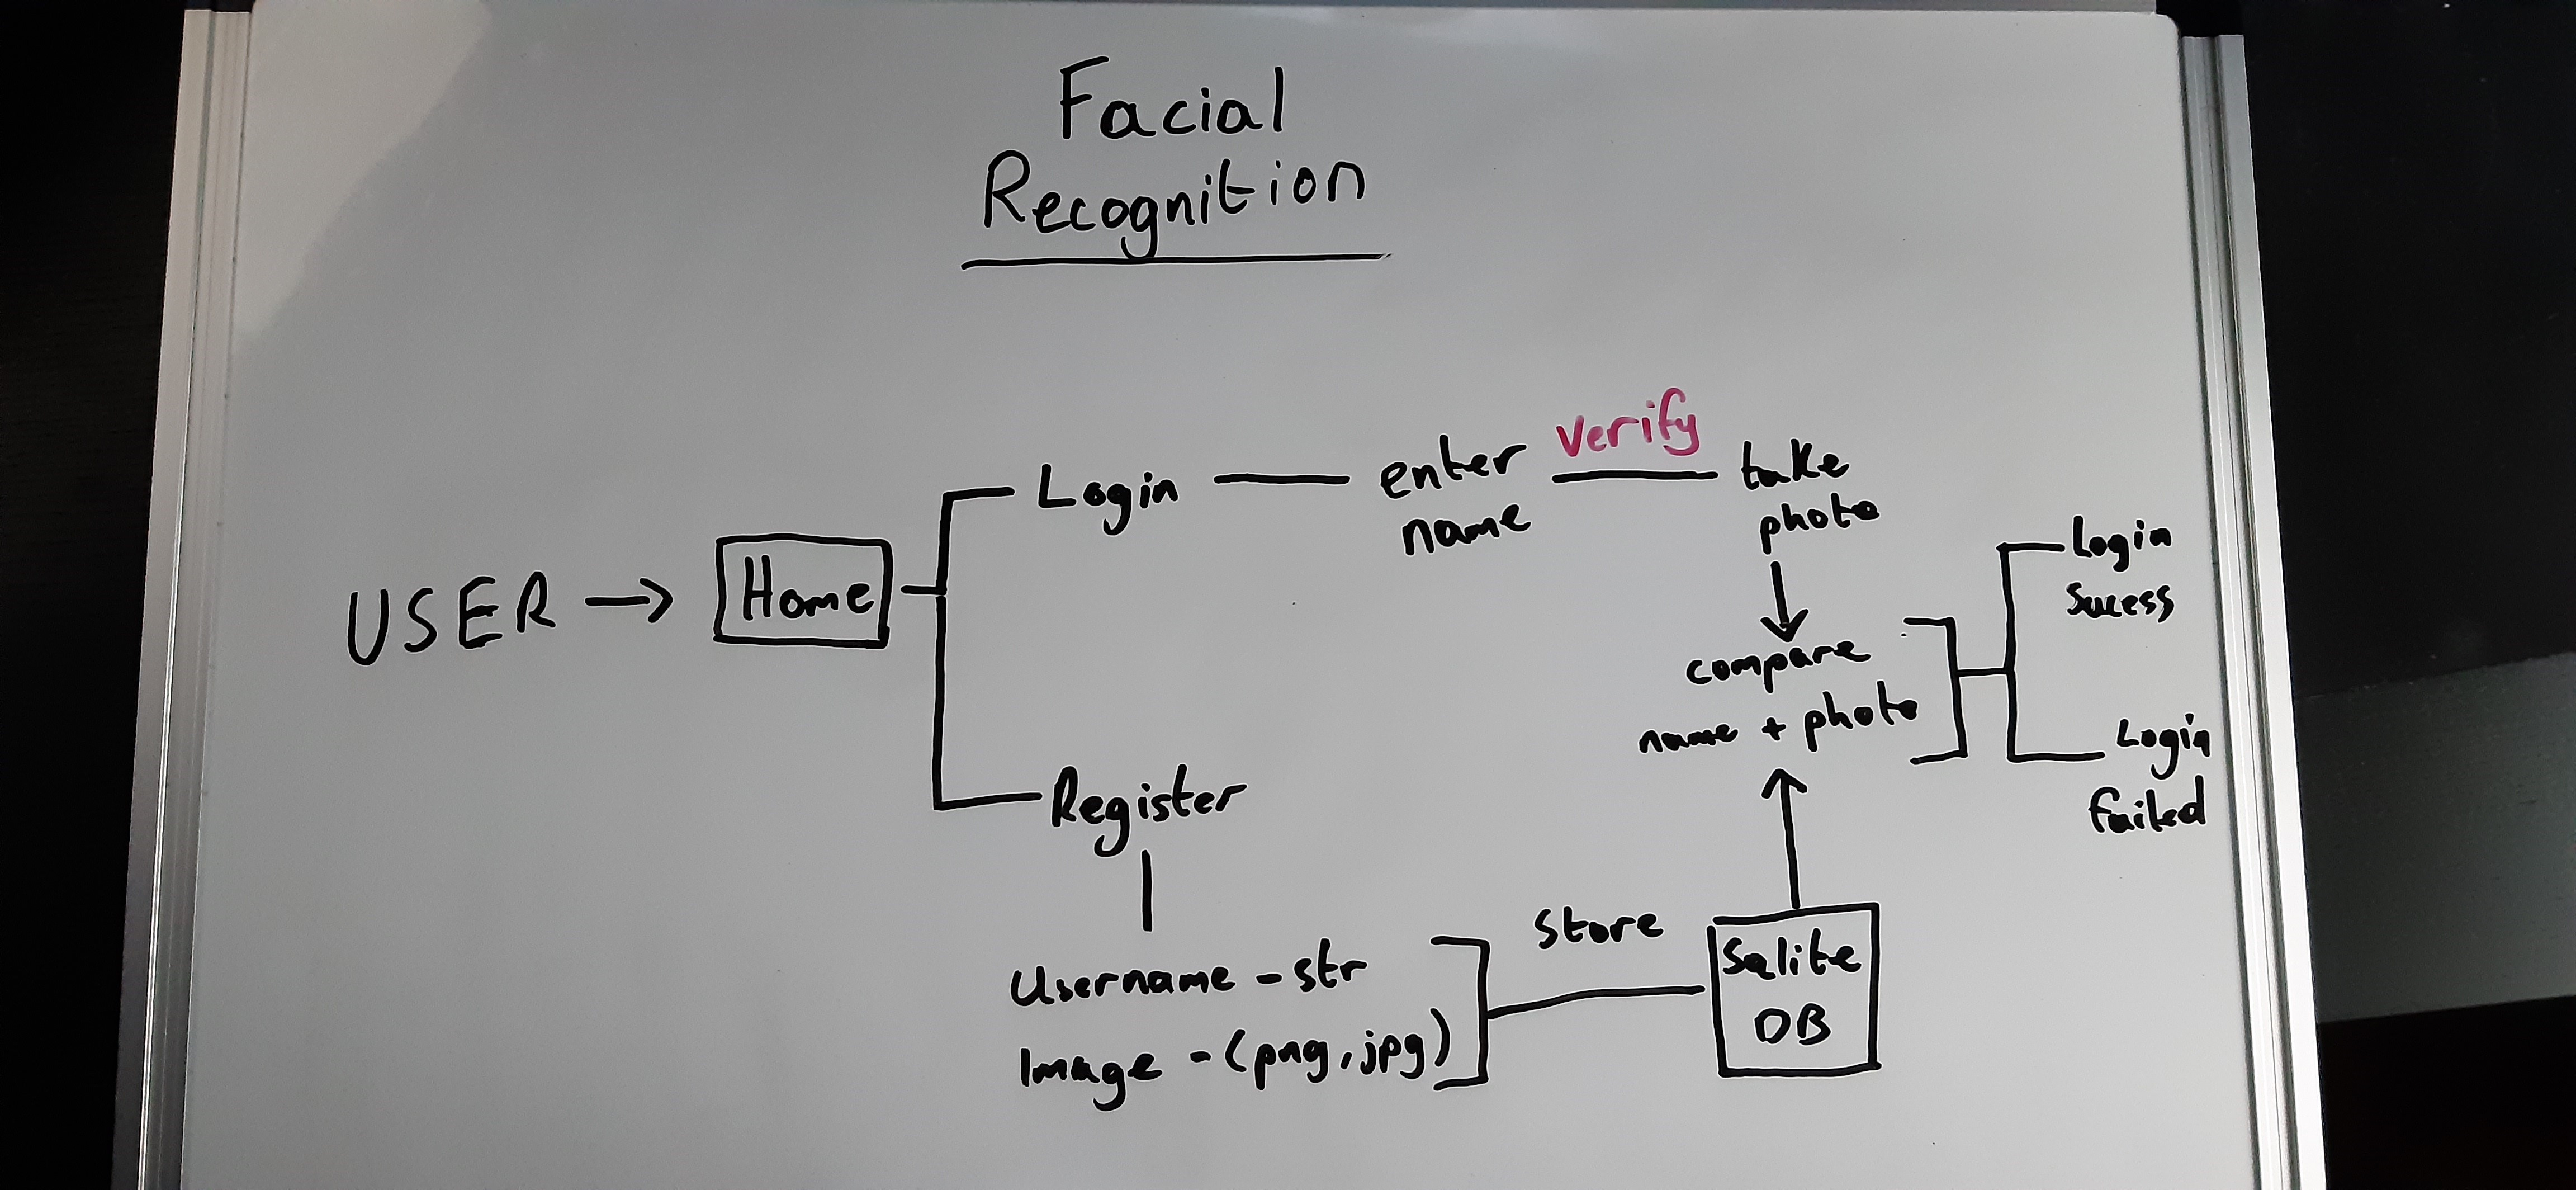
\includegraphics[scale = 0.1]{document/diagram1.jpg}
The thought we had in mind for this project was for companies to use our Register and Login software and enhance it to suit their needs.This software can be easily tailored from colour to design with customer request.
The UI design is located on one CSS file. This makes for updating style simple and quick to achieve.
The python and html files are formatted for ease of navigation. The order of the files are simple and understandable. This makes for an easier approach to edit specific files.

\begin{flushleft}
\newpage
\section{Design Methodology}
After trial and error this is the design we settled on. As you can see the design if very simple and clear. We thought about adding more to the pages like a template website but decided on "a less is more" approach to the design.

\textbf{\underline{Home Screen}}
\newline
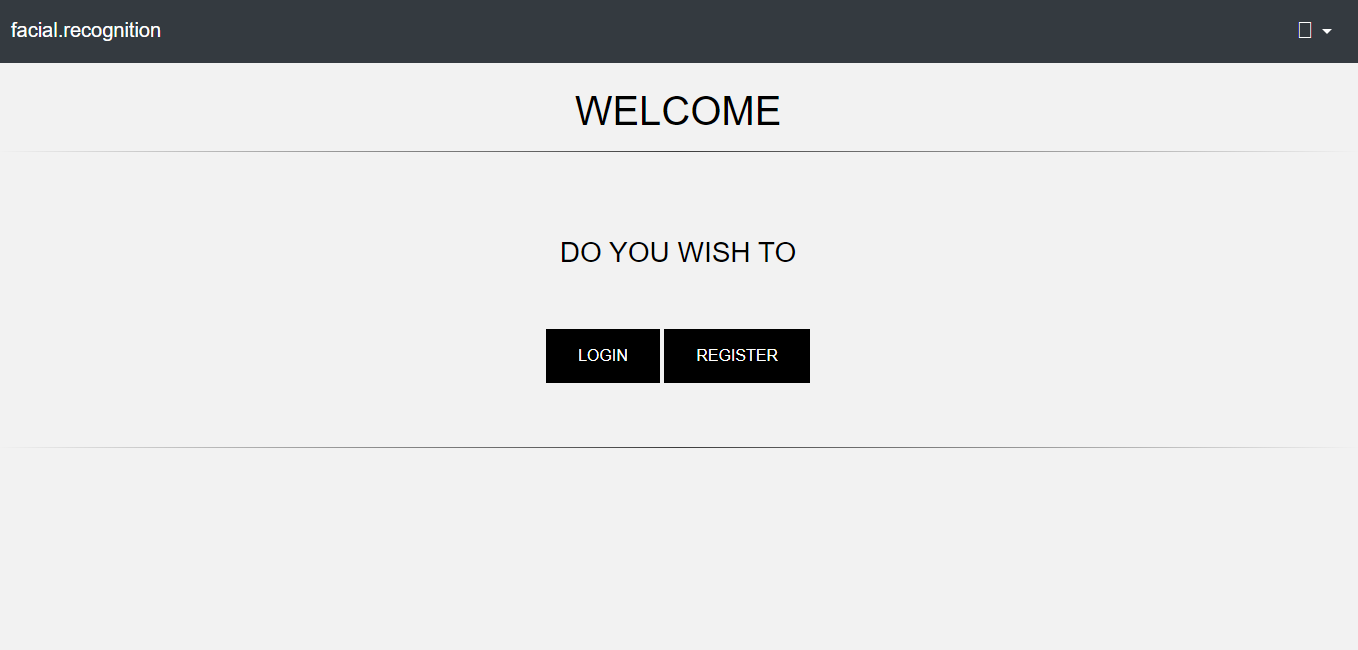
\includegraphics[scale = 0.27]{document/WelcomeScreen.PNG}
\newline\newpage
\textbf{\underline{Login Screen}}
\newline
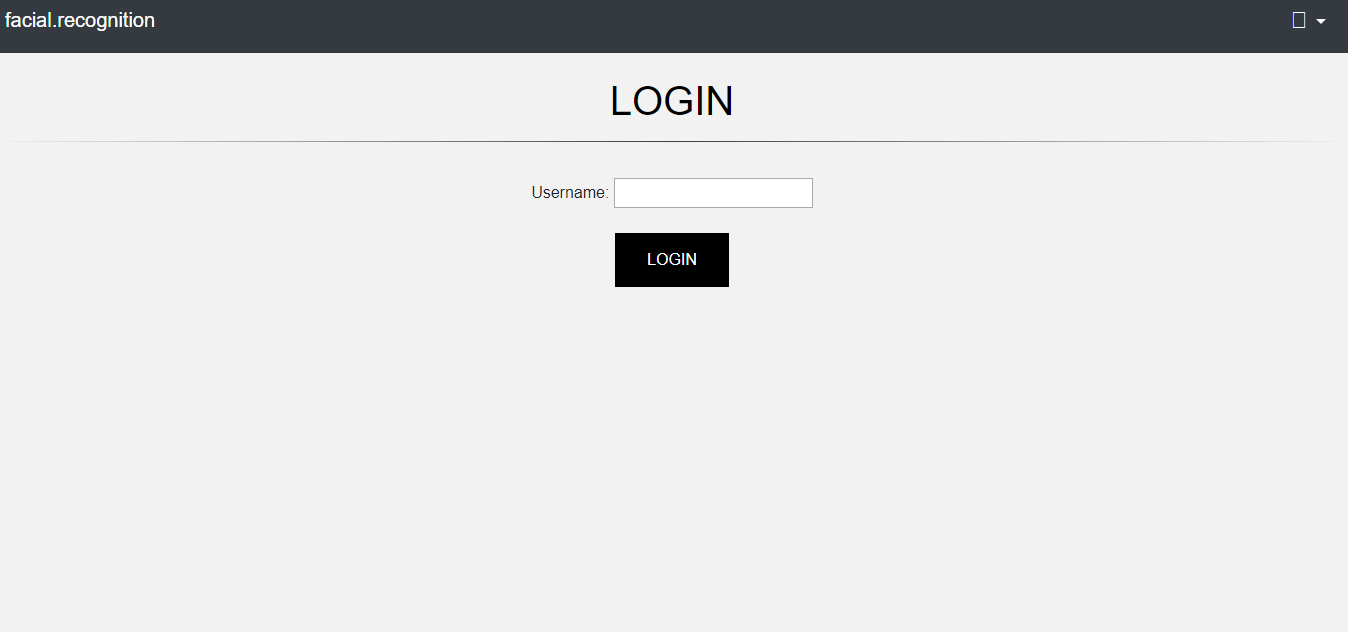
\includegraphics[scale = 0.27]{document/Login.PNG}
\newline
\textbf{\underline{Register Screen}}
\newline
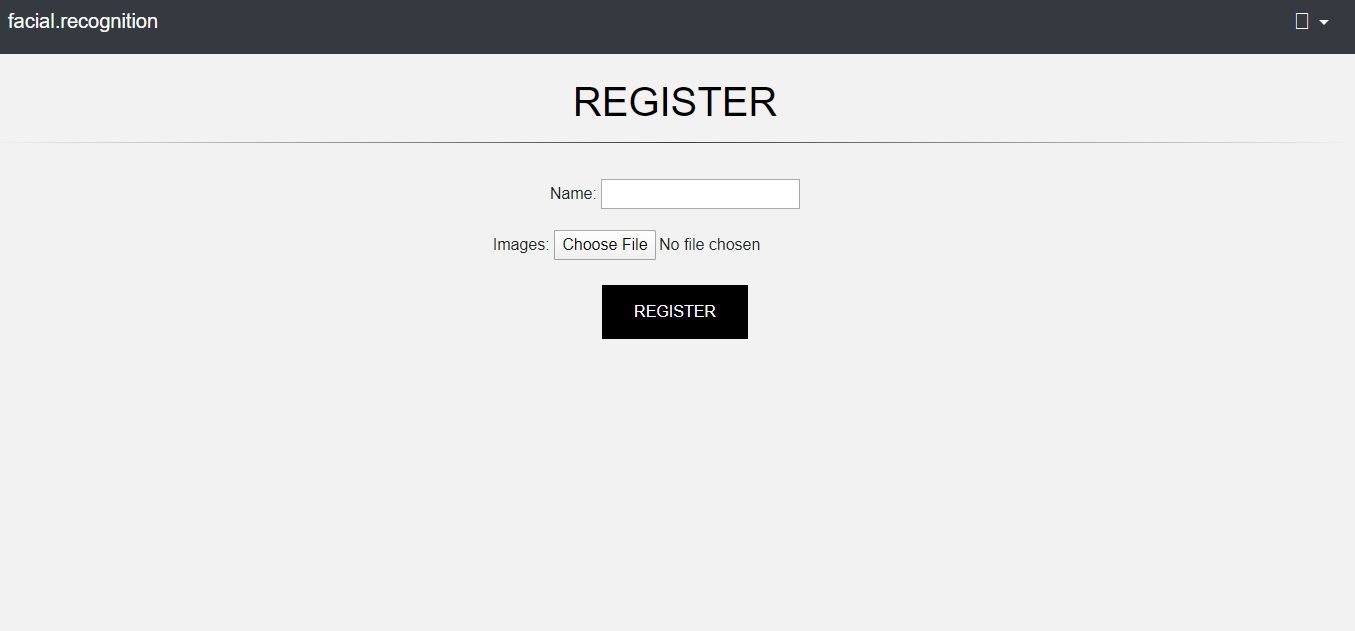
\includegraphics[scale = 0.27]{document/Register.PNG}
\label{fig:WebsiteImages}\newline
\section{Features}
\textbf{\underline{Features Included}} \newline
\textbullet{ Ability to Create a user and upload Profile picture to database}\newline
\textbullet{ Ability to Login using facial Recognition and username}\newline
\textbullet{ Once logged in the user will be displayed with a welcome message}\newline
\newpage
\section{Limitations and Bugs}
As with any programming project we encountered a plethora of bugs and limitations whilst working on this project. The most frustrating one of all was in the initial stages of the project. We had chosen to work with the \textbf{Flask} framework and had a problem with taking an image on the web page using javascript, encoding the image and sending it to our database via Ajax. This problem that we had set us back for a while until we ultimately decided to swap framework to \textbf{Django}. 

Within a few days of making the switch we managed to get our images uploading to a database and then setting up the routes for the other links in our web application.

Another bug we had encountered was an Index out range error whenever an image that did not have a recognisable face on it was loaded in, but it was tackled with simple try catch statement.

\section{Testing Plans}
We went through extensive testing whilst making this project. Every commit that was uploaded to our repository was tested beforehand before the commit.
Testing played a vital role in the production of our project. We had to make sure each small part was tested so the user experience would be up to standard. We found problems along the way whilst making of the project. One of these problems we encountered was the upload of an image. Through White Box Testing we discovered and fixed the errors we had. We also use a Black Box Testing approach to see what the user experience was like on a user that wasn't apart of the production group. This gave us insight into what we need to improve on.  

\section{Recommendation for Future Development}
For future development we will take on board everything we learned whilst doing this project. The team enjoyed the challenge of working with and learning a new language. This is something we can carry over to future development.

We now know even with extensive testing you can still hit many roadblocks along the way. Our experience of this was the framework. At the start we decided on using flask as our framework but we encountered multiple problems with our database and images. With this in mind we made the choice to switch to \textbf{Django}. This decision was made for the better of the project and once changed the project came together quickly. These types of problems will be beneficial for us in the future. Our learning of GitHub will be useful in the future. Through various lectures we learned how to use Issues on GitHub this made dealing with problems more manageable.


\section{Conclusions}
To conclude, \newline
The making of this project proved to be no easy task.Through making this project each of us learnt and improved various skills, whether it be improved communication skills, working as a team, design or coding ability. After finishing the project and looking back we feel we could have done better in some areas. For example we could have researched more into certain areas like the database or framework. This however gave us challenges to overcome. We now know how to deal with these types of problems if they were to occur in the future when we are working professionally as software developers.

\section{Acknowledgements}

\underline{\url{https://www.fullstackpython.com/table-of-contents.html}}
\newline
\underline{\url{https://www.fullstackpython.com/django.html}}
\newline
\underline{\url{https://www.fullstackpython.com/flask.html}}
\newline
\underline{\url{https://www.sqlalchemy.org/}}
\newline
\underline{\url{https://www.pythonpool.com/face-detection-using-opencv-and-python/}}
\newline
\newline
\textbf{face\_recognition library}
\underline{\url{https://github.com/ageitgey/face\_recognition/issues/175}}
\newline
\newline
\textbf{Django File Uploading:}
\underline{\url{https://docs.djangoproject.com/en/3.0/topics/http/file-uploads/}}
\newline

\underline{\url{https://medium.com/@muehler.v/node-js-opencv-for-face-recognition-37fa7cb860e8}}
\newline

\textbf{Directory Traversal in Python}
\underline{\url{https://www.pythoncentral.io/how-to-traverse-a-directory-tree-in-python-guide-to-os-walk/}}
\newline
\newline
\textbf{Sentdex}
\newline
\underline{\url{https://www.youtube.com/channel/UCfzlCWGWYyIQ0aLC5w48gBQ}}

\end{flushleft}
\end{document}
